% -*- mode: LaTeX-mode; eval: (visual-line-mode t); -*-

\PassOptionsToPackage{twoside=false}{geometry}
\documentclass[10pt,nonacm,natbib=false]{acmart}
\usepackage{amsmath}
\usepackage{listings}
\lstset{%
  basicstyle=\ttfamily\small,
  keywordstyle=\bfseries,
  columns=fullflexible,
  morekeywords={elim,by,apply,rewrite},
  frame=single,
  showstringspaces=false
}
\usepackage{url}
\usepackage{color}
\usepackage{xcolor}
\usepackage{hyperref}
\hypersetup{
    colorlinks=true,      % Set to false to disable coloring of links
    linkcolor=black,      % No color for internal links
    urlcolor=black,       % No color for URLs
    pdfborder={0 0 0}     % Remove borders around links
  }
\usepackage{graphicx}  
\usepackage{dashrule} 

\title{Project ``Proof Explainer''}
\subtitle{Advancing Proof Comprehension}
\date{\today} % Removes date from \maketitle
\author{Vadim Zaliva}
\email{vadim@zaliva.org}

\begin{document}

\maketitle

\section*{The Problem}

Formal proofs using Proof Assistants such as Rocq\footnote{formerly
  known as Coq Proof Assistant}, Lean, and Isabelle have become important design
artefacts of modern high-assurance software systems. Along with the
traditional source code base, proof scripts must be reviewed,
documented, and maintained. As different groups of proof engineers
work on them over time, proof scripts' documentation and overall
readability become crucial.

Unfortunately, proof scripts are generally not easily
human-readable. Consider the following example of a formal proof of
Gauss' Formula from Coq textbook \cite{mahboubi2021mathematical}, and
compare it with the proof from a classical mathematics textbook
\cite{roberts2014introduction}, shown in Appendix~\ref{sec:textbookproof}.

\begin{lstlisting}
Example gauss n :
  \sum_(0 <= i < n+1) i = n * n+1 %/ 2.
Proof.
  elim: n =>[|n IHn]; first by apply: big_nat1.
  rewrite big_nat_recr //= IHn addnC -divnMDl //.
  by rewrite mulnS muln1 -addnA -mulSn -mulnS.
Qed.
\end{lstlisting}

The difficulty of human comprehensibility goes beyond the obscure
syntax and is inherent to tactic languages. Each tactic operates on an
implicit proof state, which is invisible unless you step through the
script in the proof assistant. Even if the proof state is available,
it could be large, making it difficult to focus on the relevant part
of each step. Some features of proof assistants allow for writing more
human-readable proofs, but proof writers often ignore them in favour
of brevity and expediency. One example is use automatic variable
naming which is convenient, but makes proofs less
readable. Additionally, while tactic languages support some
structuring of the proof script to reflect the branching of the proof
tree, these features are not always rigorously used by human proof
writers, and their expressivity is limited.

In any sizeable proof development, the proof is structured into
theorems, lemmas, and corollaries, dividing it into more
comprehensible fragments.  Thus, when explaining a particular theorem,
it is beneficial to utilise the meaning of the auxiliary lemmas it
relies on and present the current proof using high-level intuitive
descriptions of these lemmas. For example, it is helpful to recognise
that an auxiliary lemma stating
$\forall a, b, c \; (a + (b + c) = (a + b) + c)$ expresses the
\textit{associativity of addition} and to refer to it using this more
accessible description.

\section*{Proposal}

We propose to develop a tool to explain and document Rocq proofs with
the help of LLMs. When applied to an already proven lemma, the Proof
Explainer will produce standalone documentation or annotated and
restructured for readability proof script. It could be made accessible
via a simple web interface or integrated into the proof assistant’s
IDE (e.g. as a VS Code plugin). The command line version could be used
in a build or continuous integration process to generate online
documentation or to annotate proof scripts.

It would be immediately helpful to a wide array of users. Professional
proof engineers could use it to examine and understand existing proof
code bases. The generated documentation could be used to onboard new
team members and conduct code reviews. It would immediately benefit
students of formal methods and proof engineering by allowing to break
down and understand the intricacies of existing proofs. It could be an
invaluable educational tool for learning best practices and building
confidence in engaging with real-world proof codebases.

\section*{The approach}

While current LLMs already provide a decent explanation of simple,
self-contained proofs, as shown in our Gauss's formula example in
Appendix~\ref{sec:explained}, they struggle with larger proofs that
use auxiliary lemmas, third-party libraries, and custom
notations. Another reason they perform much better on simple textbook
proofs is that these have been published before, discussed online, and
were likely included in the training corpus.

The key observation is that explaining proofs requires insight into
the proof state, as maintained by a proof assistant. Our tool will
integrate a proof assistant to access this information. We can use
proof assistant APIs to disambiguate syntax and access the per-step
proof state, definitions, and types. When proof automation is used, we
can unroll the automation steps to access their intermediate results.

The second insight is that current LLMs have a limit on a LLM’s
context window, and feeding the whole proof along with all related
definitions is impractical. This calls for carefully curating the
information supplied to the model at each reasoning step. We can
supply only necessary definitions, strip irrelevant parts of the proof
context, or supply only the calculated diffs between the proof states.

Additionally, we can leverage different models and arbitrage or verify
their results. Using the well-established “AI agents” approach, we can
split reasoning into several steps and process each via separate LLM
queries.

Finally, we can perform multi-pass elaboration for projects containing
reusable lemmas, first processing the auxiliary lemmas and later using
AI-generated summaries of already processed lemmas accessible via
retrieval-augmented generation (RAG) or similar techniques.

In the initial project stage, we would focus first on the Rocq proof
assistant, which is mature and has good automation means (LSP protocol
server, plugin API, and command-line tools). Many Rocq proofs are
published as open source, which we can use for training, testing, and
validation. Our preliminary experiments show that popular LLM models
like OpenAIi o1 and Anthropic Claude 3.5 Sonnet can perform basic Rocq
proof elaboration, which we can use as a baseline.

\section*{Key Differentiators and Related Work}

Several recent projects have used LLMs for formal proofs. For example,
\cite{DBLP:conf/kbse/LuD024, DBLP:journals/corr/abs-2410-14835, DBLP:conf/nips/WuJLRSJS22, DBLP:conf/icml/YangD19, DBLP:journals/corr/abs-2403-12627, DBLP:conf/kbse/KozyrevSKP24, DBLP:conf/nips/YangSGCSYGPA23, DBLP:conf/emnlp/WangZJPDPZ24}.  Most attempt to synthesise
proofs from scratch or aid in repairing existing proofs. Given the
current early state of LLMs, these are ambitious goals. We believe
that to reach the ultimate goal of fully automated proof synthesis,
merely promoting or guiding existing models is insufficient, and a
deeper integration into the LLM reasoning process is required, as, for
example, proposed in \cite{park2024grammaraligneddecoding}. The
required approaches would likely be costly, with prices comparable to
training new LLMs. Our goals are more modest, and we are trying to
play on the strength of existing models in knowledge summarisation and
presentation, where they are already showing promising results.

\section*{Budget \& Estimates}

This is a relatively small-scale project, estimated to take 6 to 8
months. The work is roughly evenly split between engineering (such as
integration with proof assistants and LLM APIs) and research
(experimenting with different LLMs, prompting strategies, implementing
retrieval-augmented generation (RAG) techniques, etc.), making a
dedicated full-time research engineer essential for effective
execution.

While undergraduate and graduate students may contribute, their
involvement will be on a voluntary or part-time basis, providing
additional support in both engineering and research aspects. The
involvement of the PI (and potentially a co-PI) is provided at no
cost.

The estimated budget of approximately \$20K primarily covers the
salary of the research engineer and LLM usage fees.

\appendix

\newpage
\section{Mathematical Textbook Proof of Gauss' Summation Formula}

\label{sec:textbookproof}

\begin{figure}[h]
\fbox{
  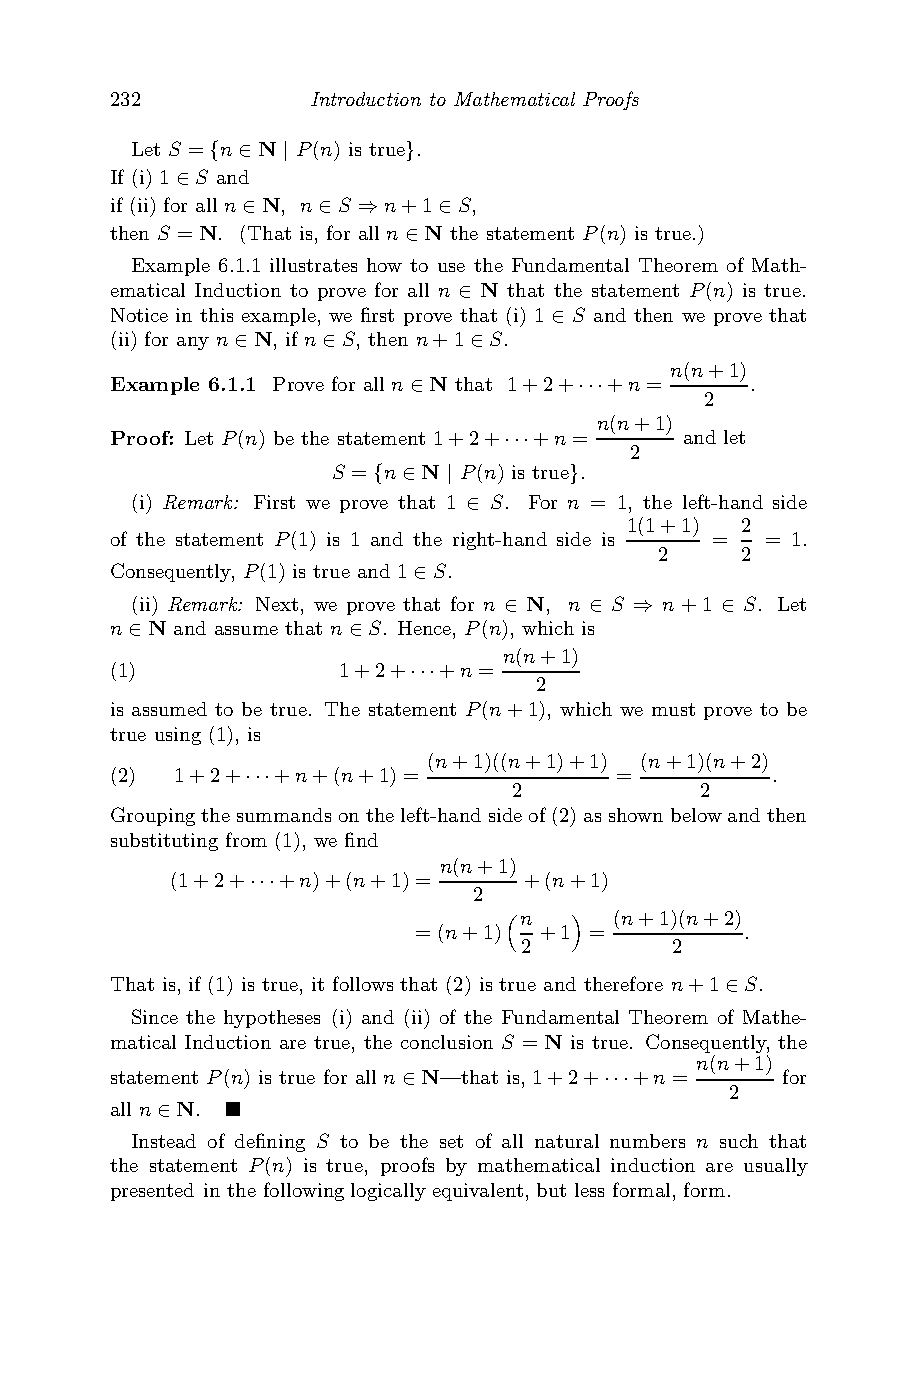
\includegraphics[page=1, trim=0cm 4.4cm 0cm 6cm, clip, width=\textwidth]{page236.pdf}
  }
  \caption{A ``pen and paper'' proof of Gauss' Summation Formula from \cite{roberts2014introduction}}
\end{figure}
  
\newpage
\section{Appendix: LLM-Explained Rocq Proof of Gauss's Summation Formula}
\label{sec:explained}

The following explanation is produced by ChatGPT \textit{o3-mini-high}
model using the following prompt.

\begin{quotation}
  \textit{Explain this proof. In addition to explaining the
    mathematical proof, provide a step-by-step explanation of the
    proof script. Give me the explanation in LaTeX format. [proof script text]}

\end{quotation}

\noindent The models' \LaTeX\ output contained some poorly formatted
maths and was manually cleaned. The artificially introduced math
notation $(n.+1)$ for the successor of natural numbers was simplified
to $(n+1)$.

It should also be noted that the classic formulation of Gauss's
formula sums all numbers starting from $1$, and consequently, most
textbook proofs proceed by induction with $1$ as the base case. The
Rocq formalisation we used starts the summation from $0$ and proceeds
by induction with the base case $0$. While both formulations are
equivalent and both proof approaches yield the same result, this
difference between classic mathematics and formal proofs in Rocq is
worth highlighting.

\noindent\hdashrule[0.5ex]{\textwidth}{1pt}{1pt}

In this appendix we explain the following Coq/SSReflect proof of the formula
\[
\sum_{i=0}^ {n} i = \frac{n(n+1)}{2},
\]
which is the well-known result for the sum of the first \( n \) natural numbers.

\subsection*{Proof Script}
\begin{lstlisting}
Example gauss n :
  \sum_(0 <= i < n+1) i = n * n+1 %/ 2.
Proof.
  elim: n =>[|n IHn]; first by apply: big_nat1.
  rewrite big_nat_recr //= IHn addnC -divnMDl //.
  by rewrite mulnS muln1 -addnA -mulSn -mulnS.
Qed.
\end{lstlisting}

\subsection*{Step-by-Step Explanation}

\paragraph{1. Statement of the Theorem:}
The goal is to prove that
\[
\sum_{i=0}^{n} i = \frac{n(n+1)}{2}.  
\]
Here, the notation \( n+1 \) denotes the successor of \( n \) (i.e. \( n+1 \)), and the summation \(\sum_{i=0}^{n}\) is taken over the integers \( 0, 1, \dots, n \).

\paragraph{2. Proof by Induction:} 
The proof proceeds by induction on \( n \), as initiated by the command:
\begin{verbatim}
elim: n =>[|n IHn];
\end{verbatim}
This command splits the proof into two cases:
\begin{itemize}
    \item The \emph{base case} where \( n = 0 \).
    \item The \emph{inductive step} where one assumes the statement for \( n \) (captured by the identifier \verb|IHn|) and then proves it for \( n+1 \).
\end{itemize}

\paragraph{3. Base Case (\( n = 0 \)):}
For \( n = 0 \), the summation becomes
\[
\sum_{0 \le i < 0+1} i = \sum_{i=0}^{0} i = 0.
\]
The right-hand side is
\[
\frac{0 \times 1}{2} = 0.
\]
Thus, the equality holds. The tactic:
\begin{verbatim}
first by apply: big_nat1.
\end{verbatim}
applies the lemma \texttt{big\_nat1}, which establishes that the sum over a singleton range is equal to the sole element in that range (here, \(0\)).

\paragraph{4. Inductive Step:}
Assuming the induction hypothesis (IHn):
\[
\sum_{i=0}^{n} i = \frac{n(n+1)}{2},
\]
we must show that
\[
\sum_{0 \le i < (n+1)+1} i = \frac{(n+1)(n+2)}{2}.
\]

\paragraph{5. Decomposing the Sum:}
The tactic:
\begin{verbatim}
rewrite big_nat_recr //= IHn addnC -divnMDl //.
\end{verbatim}
performs several operations:
\begin{itemize}
    \item \texttt{big\_nat\_recr} rewrites the extended summation 
    \[
    \sum_{0 \le i < (n+1)+1} i
    \]
    as the sum of the previous range plus the final term:
    \[
    \left(\sum_{i=0}^{n} i\right) + (n+1).
    \]
    \item The \texttt{//=} notation triggers automatic simplification.
    \item \texttt{IHn} replaces \(\sum_{i=0}^{n} i\) with \(\frac{n(n+1)}{2}\) by the induction hypothesis.
    \item \texttt{addnC} utilises the commutativity of addition to rearrange terms.
    \item \texttt{-divnMDl} manages the division by \( 2 \), preparing the expression for the subsequent algebraic manipulation.
\end{itemize}

\paragraph{6. Algebraic Simplification:}
The final rewriting step is given by:
\begin{verbatim}
by rewrite mulnS muln1 -addnA -mulSn -mulnS.
\end{verbatim}
This step uses a series of algebraic rewrite rules:
\begin{itemize}
    \item \texttt{mulnS} rewrites multiplication involving the successor, for instance, expressing \((n+1)(n+1)\) as \( n(n+1) + (n+1) \).
    \item \texttt{muln1} emphasises that multiplying by \( 1 \) does not change a number.
    \item \texttt{-addnA} applies the associativity of addition.
    \item \texttt{-mulSn} and \texttt{-mulnS} further manipulate the multiplicative structure.
\end{itemize}
Together, these rewrites confirm that:
\[
\frac{n(n+1)}{2} + (n+1) = \frac{(n+1)(n+2)}{2},
\]
which is exactly the form required to complete the inductive step.

\paragraph{7. Conclusion:}
Since both the base case and the inductive step have been established, by the principle of mathematical induction the formula
\[
\sum_{i=0}^{n} i = \frac{n(n+1)}{2}
\]
holds for all natural numbers \( n \).


\newpage
\bibliographystyle{acm}
\bibliography{whitepaper}


\end{document} 

